\chapter{Analytical Model}
\label{ch:analyticalmodel}

\section{Basics of the quasiclassical model}
\begin{figure}
\centering
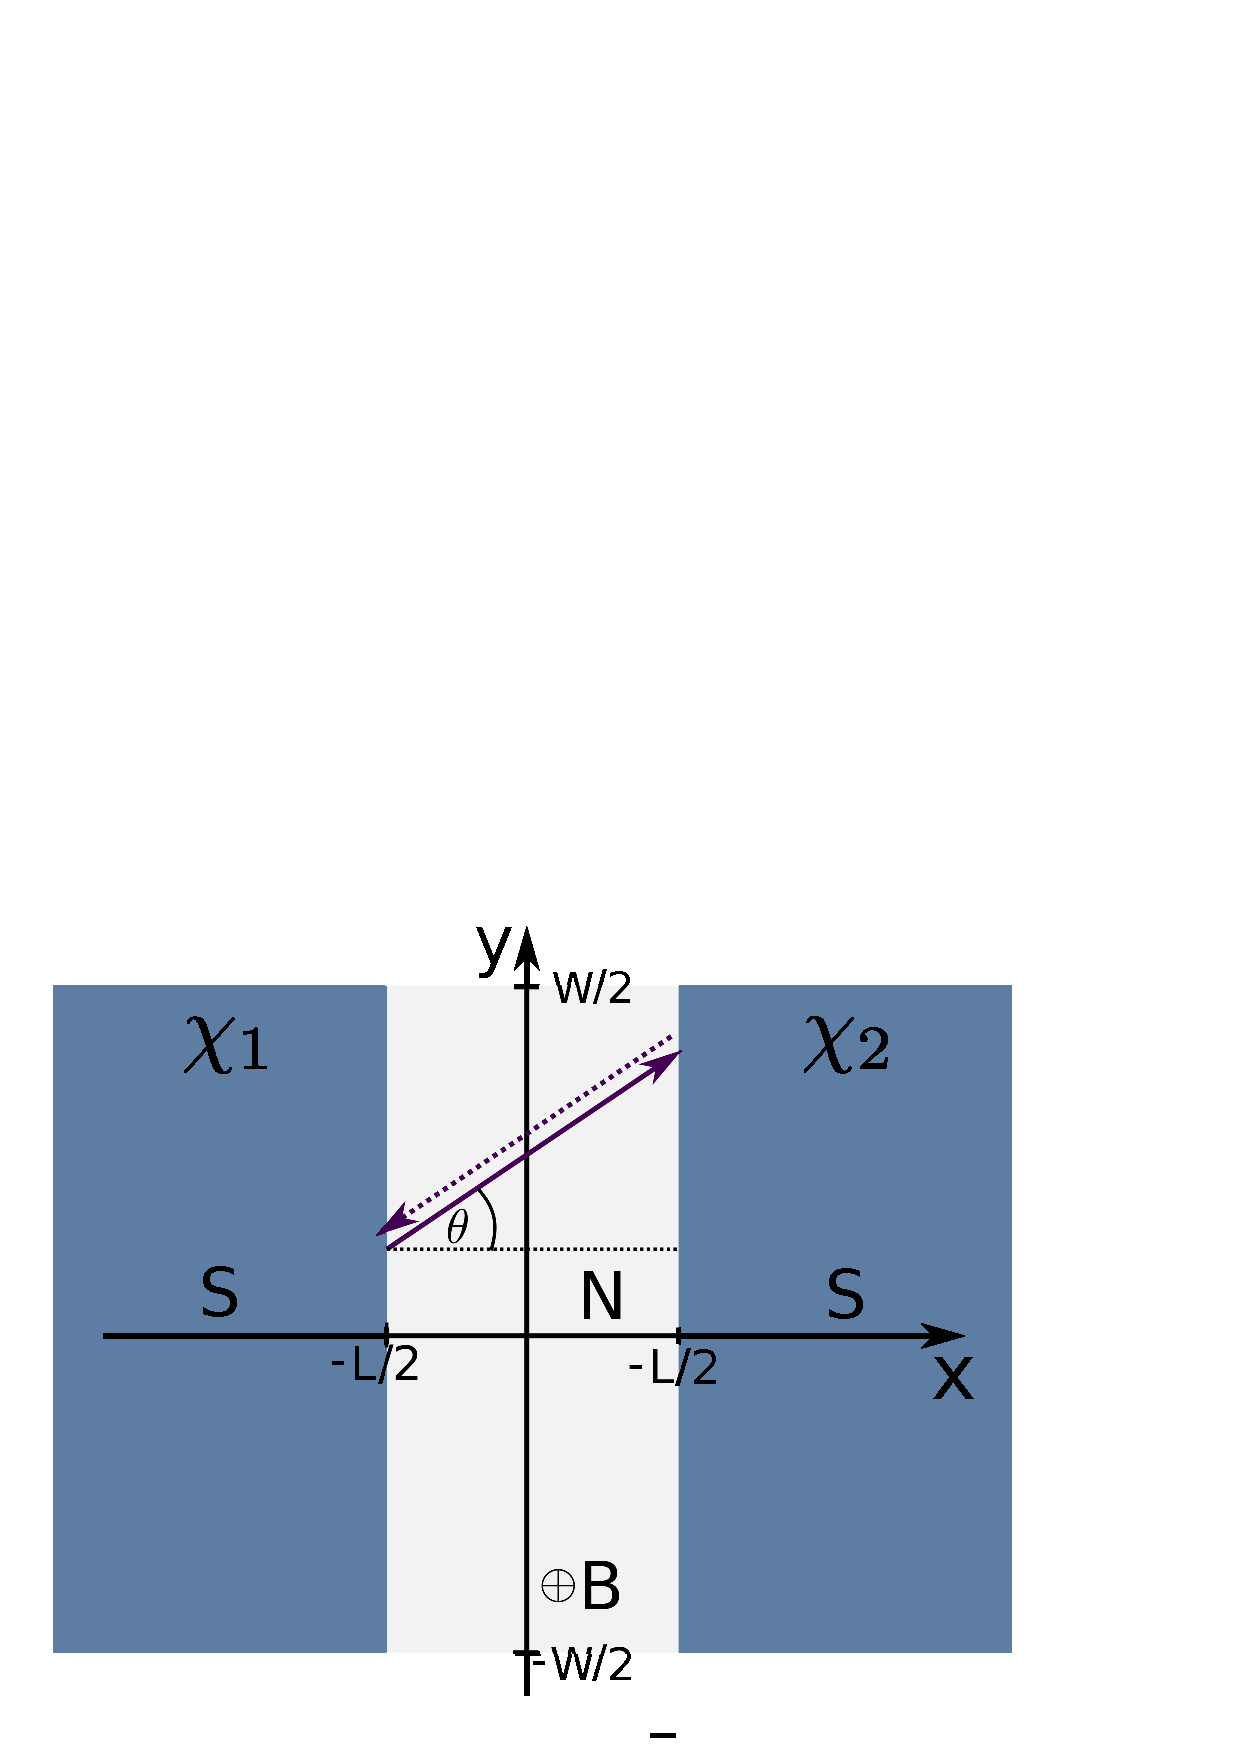
\includegraphics[width=0.6\textwidth]{figure/analyticalmodel/sns_junction.pdf}
\caption{Schematic representation of a short and wide SNS junction.}
\label{fig:sns_schematic}
\end{figure}

In figure \ref{fig:sns_schematic} a schematic SNS junction is depicted. The setup is two dimensional with width $W$ and length $L$. The NS-interfaces are parallel to the $y$-axis and are placed at $x = \pm L/2$. Each of the superconducting leads has a phase $\chi_{1}$ and $\chi_{2}$ and the overall phase difference is $\chi = \chi_{1} - \chi_{2}$.
The superconducting gap parameter is only present in the superconducting leads and zero in the normal region and can be expressed as
\begin{equation}
\Delta\left( x \right) = |\Delta| e^{\chi_1} \Theta\left(-L/2 -x \right) + |\Delta| e^{\chi_2} \Theta\left(x-L/2 \right) 
\end{equation}
The aim is to express the current through the junction using a quasiclassical approach. In this approach, the Andreev bound states are assosiated with straight trajectories connecting the superconducting leads. The superconducting current density is expressed in terms of these trajectories. 

Now, check if this quasiclassical approach is valid. What are preliminary assumptions about the system?

The presence of magnetic field will lead to a bending of the trajectories due to the Lorentz force. Depending on the strength of magnetic field $B$ and the Fermi velocity the radius of this curve is 
\begin{equation}
r_B = ???
\end{equation}
%TODO add the formula for cyclotron radius
In order to justify the assumption of straight trajectories, either the magnetic field has to be weak enough or the Fermi wavelength has to be short enough. Because then, the cyclotron radius $r_B$ is simply much smaller than the sample length $L$.



Assumptions for model:
* Superconducting gap is stepfunction like
* ballistic sample with totally absorbing boundaries
* fermi wave length is small compared to other length scales in the system: 
** cyclotron radius $r_B \gg L$, $L$ is the length of the sample --> straight trajectories is alright as an assumption
** low temperature limit: $k_B T \ll \hbar v_F / L$ 
** coherence length: $\lambda_F \ll \zeta$
** magnetic field penetration depth $\lambda_F \ll \lambda_L$
** sample length: $\lambda_F \ll L$
* both charge carrier density and chemical potential in BLG are sufficiently high, therefore single band model is alright
* Following approach of Zagoskyn (with Eilenberger equations): formula for $I_c$. Each contribution to critical current depends on the length of the trajectory and on the phase gained along it

In \ref{fig:sns_schematic} the schematics of a SNS junction is depicted. The junction consists of two superconducting leads and a normal metal layer in the middle. 

\begin{figure}
\centering
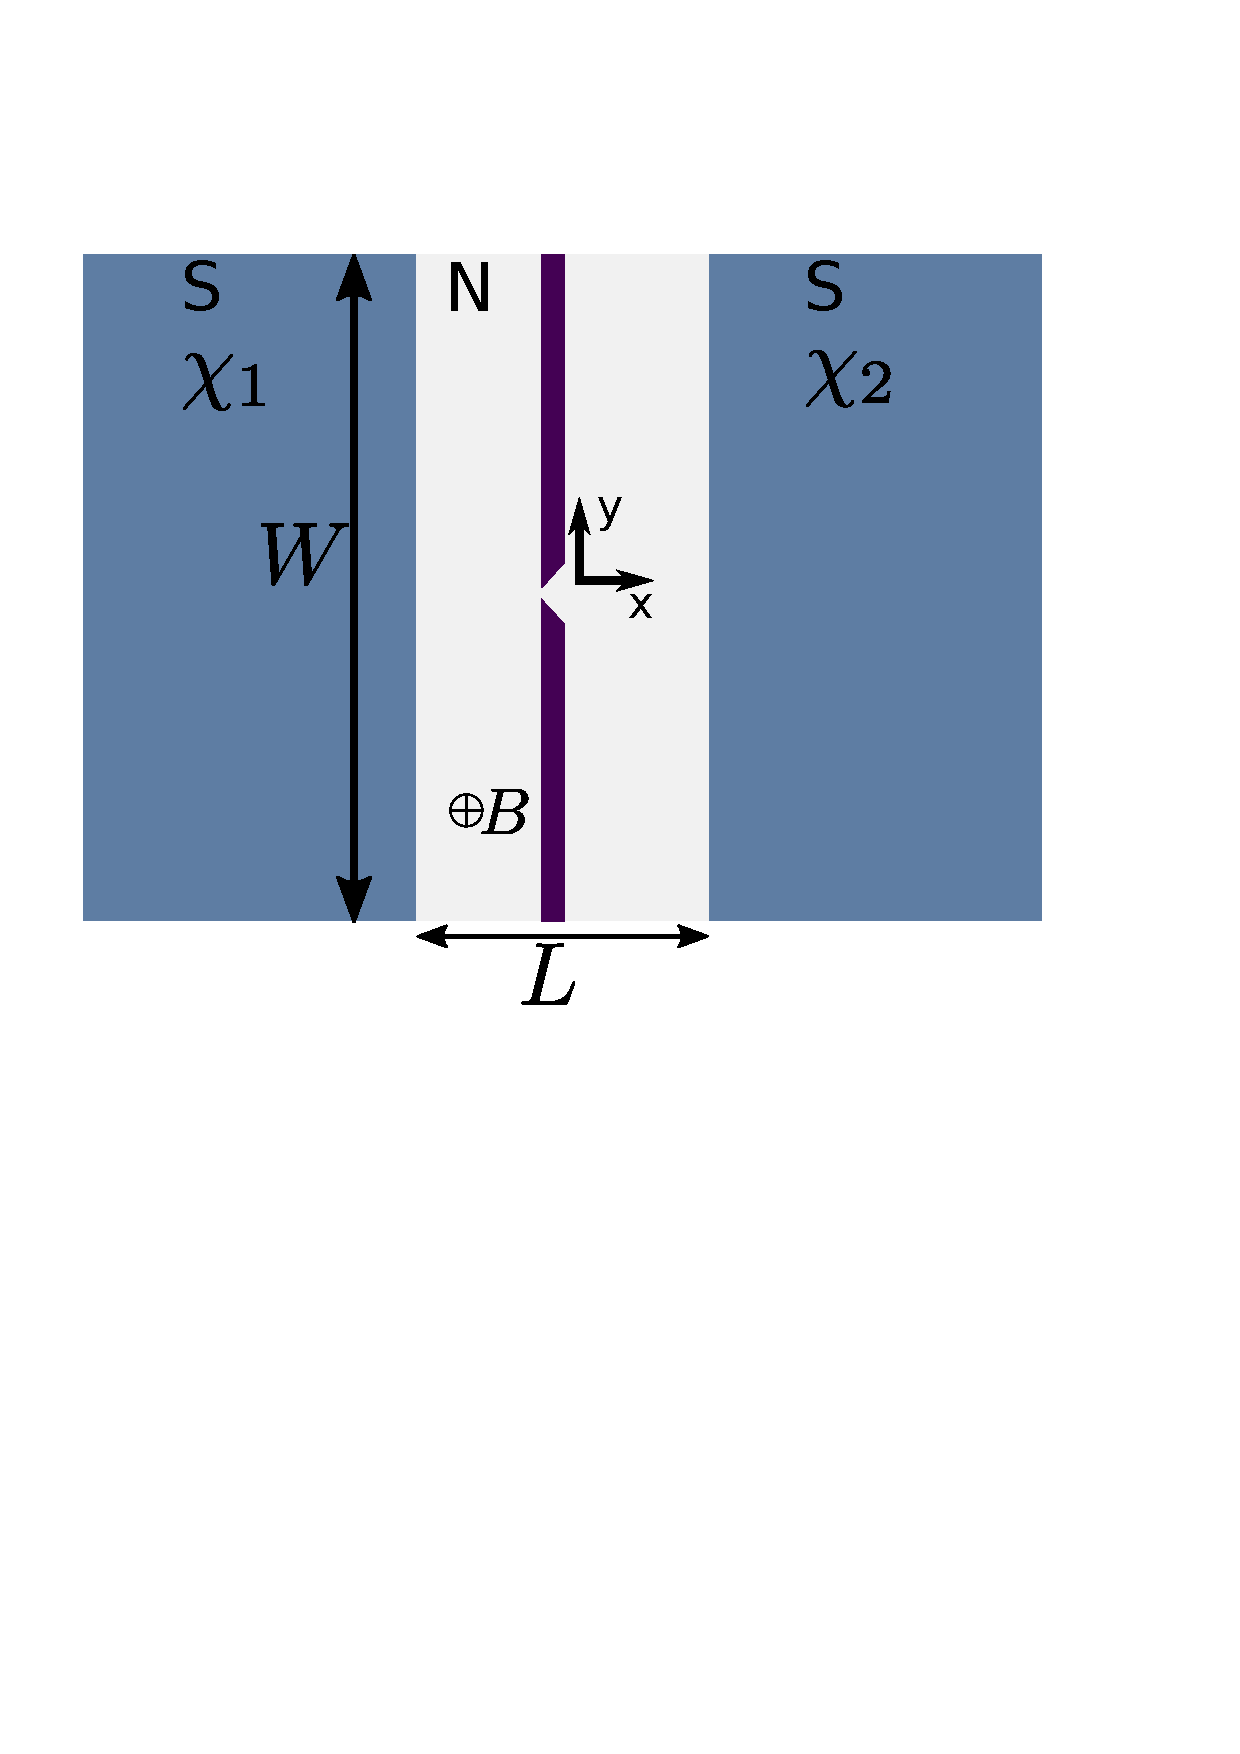
\includegraphics[width=0.6\textwidth]{figure/analyticalmodel/qpc_sns_junction.pdf}
\caption{Schematic representation of a short and wide SNS junction with QPC setup.}
\label{fig:qpc_sns_schematic}
\end{figure}